%%
%% This is file `sample-sigconf-authordraft.tex',
%% generated with the docstrip utility.
%%
%% The original source files were:
%%
%% samples.dtx  (with options: `all,proceedings,bibtex,authordraft')
%% 
%% IMPORTANT NOTICE:
%% 
%% For the copyright see the source file.
%% 
%% Any modified versions of this file must be renamed
%% with new filenames distinct from sample-sigconf-authordraft.tex.
%% 
%% For distribution of the original source see the terms
%% for copying and modification in the file samples.dtx.
%% 
%% This generated file may be distributed as long as the
%% original source files, as listed above, are part of the
%% same distribution. (The sources need not necessarily be
%% in the same archive or directory.)
%%
%%
%% Commands for TeXCount
%TC:macro \cite [option:text,text]
%TC:macro \citep [option:text,text]
%TC:macro \citet [option:text,text]
%TC:envir table 0 1
%TC:envir table* 0 1
%TC:envir tabular [ignore] word
%TC:envir displaymath 0 word
%TC:envir math 0 word
%TC:envir comment 0 0
%%
%% The first command in your LaTeX source must be the \documentclass
%% command.
%%
%% For submission and review of your manuscript please change the
%% command to \documentclass[manuscript, screen, review]{acmart}.
%%
%% When submitting camera ready or to TAPS, please change the command
%% to \documentclass[sigconf]{acmart} or whichever template is required
%% for your publication.
%%
%%
% \documentclass[sigconf,authordraft]{acmart}
\documentclass[sigconf]{acmart}
%%
%% \BibTeX command to typeset BibTeX logo in the docs
\AtBeginDocument{%
  \providecommand\BibTeX{{%
    Bib\TeX}}}

%% Rights management information.  This information is sent to you
%% when you complete the rights form.  These commands have SAMPLE
%% values in them; it is your responsibility as an author to replace
%% the commands and values with those provided to you when you
%% complete the rights form.
\setcopyright{acmlicensed}
\copyrightyear{2025}
\acmYear{2025}
\acmDOI{XXXXXXX.XXXXXXX}
%% These commands are for a PROCEEDINGS abstract or paper.
\acmConference[UT MSAI: AI In Healthcare, Spring 2025]{}{January - May, 2025}{Austin, TX}
%%
%%  Uncomment \acmBooktitle if the title of the proceedings is different
%%  from ``Proceedings of ...''!
%%
%%\acmBooktitle{Woodstock '18: ACM Symposium on Neural Gaze Detection,
%%  June 03--05, 2018, Woodstock, NY}
\acmISBN{978-1-4503-XXXX-X/2018/06}


%%
%% Submission ID.
%% Use this when submitting an article to a sponsored event. You'll
%% receive a unique submission ID from the organizers
%% of the event, and this ID should be used as the parameter to this command.
%%\acmSubmissionID{123-A56-BU3}

%%
%% For managing citations, it is recommended to use bibliography
%% files in BibTeX format.
%%
%% You can then either use BibTeX with the ACM-Reference-Format style,
%% or BibLaTeX with the acmnumeric or acmauthoryear sytles, that include
%% support for advanced citation of software artefact from the
%% biblatex-software package, also separately available on CTAN.
%%
%% Look at the sample-*-biblatex.tex files for templates showcasing
%% the biblatex styles.
%%

%%
%% The majority of ACM publications use numbered citations and
%% references.  The command \citestyle{authoryear} switches to the
%% "author year" style.
%%
%% If you are preparing content for an event
%% sponsored by ACM SIGGRAPH, you must use the "author year" style of
%% citations and references.
%% Uncommenting
%% the next command will enable that style.
%%\citestyle{acmauthoryear}


%%
%% end of the preamble, start of the body of the document source.
\begin{document}

%%
%% The "title" command has an optional parameter,
%% allowing the author to define a "short title" to be used in page headers.
\title{Synthesized Conversation System for Medication Adherence}

%%
%% The "author" command and its associated commands are used to define
%% the authors and their affiliations.
%% Of note is the shared affiliation of the first two authors, and the
%% "authornote" and "authornotemark" commands
%% used to denote shared contribution to the research.

\author{Evan Jones}
\affiliation{%
  \institution{University of Texas at Austin}
  \city{Austin}
  \state{Texas}
  \country{USA}}
\email{evan_jones@utexas.edu}


%%
%% By default, the full list of authors will be used in the page
%% headers. Often, this list is too long, and will overlap
%% other information printed in the page headers. This command allows
%% the author to define a more concise list
%% of authors' names for this purpose.
\renewcommand{\shortauthors}{Jones}

%%
%% The abstract is a short summary of the work to be presented in the
%% article.
\begin{abstract}
  Adherence to medical advice such as medication prescriptions is the largest 
  barrier to succesful management of a number of conditions. We propose an 
  automated system to increase adherence via daily conversations initiated by a
  large language model (LLM).  The intention is that a conversational, friendly
  interaction should be more effective at increasing adherence than static 
  automated reminders.

\end{abstract}

% %%
% %% The code below is generated by the tool at http://dl.acm.org/ccs.cfm.
% %% Please copy and paste the code instead of the example below.
% %%
% \begin{CCSXML}
% <ccs2012>
%  <concept>
%   <concept_id>00000000.0000000.0000000</concept_id>
%   <concept_desc>Do Not Use This Code, Generate the Correct Terms for Your Paper</concept_desc>
%   <concept_significance>500</concept_significance>
%  </concept>
%  <concept>
%   <concept_id>00000000.00000000.00000000</concept_id>
%   <concept_desc>Do Not Use This Code, Generate the Correct Terms for Your Paper</concept_desc>
%   <concept_significance>300</concept_significance>
%  </concept>
%  <concept>
%   <concept_id>00000000.00000000.00000000</concept_id>
%   <concept_desc>Do Not Use This Code, Generate the Correct Terms for Your Paper</concept_desc>
%   <concept_significance>100</concept_significance>
%  </concept>
%  <concept>
%   <concept_id>00000000.00000000.00000000</concept_id>
%   <concept_desc>Do Not Use This Code, Generate the Correct Terms for Your Paper</concept_desc>
%   <concept_significance>100</concept_significance>
%  </concept>
% </ccs2012>
% \end{CCSXML}

% \ccsdesc[500]{Do Not Use This Code~Generate the Correct Terms for Your Paper}
% \ccsdesc[300]{Do Not Use This Code~Generate the Correct Terms for Your Paper}
% \ccsdesc{Do Not Use This Code~Generate the Correct Terms for Your Paper}
% \ccsdesc[100]{Do Not Use This Code~Generate the Correct Terms for Your Paper}

%%
%% Keywords. The author(s) should pick words that accurately describe
%% the work being presented. Separate the keywords with commas.
\keywords{AI, Artificial Intelligence, Large Language Model, LLM, Adherence, Medication}
%% A "teaser" image appears between the author and affiliation
%% information and the body of the document, and typically spans the
%% page.
\begin{teaserfigure}
  % 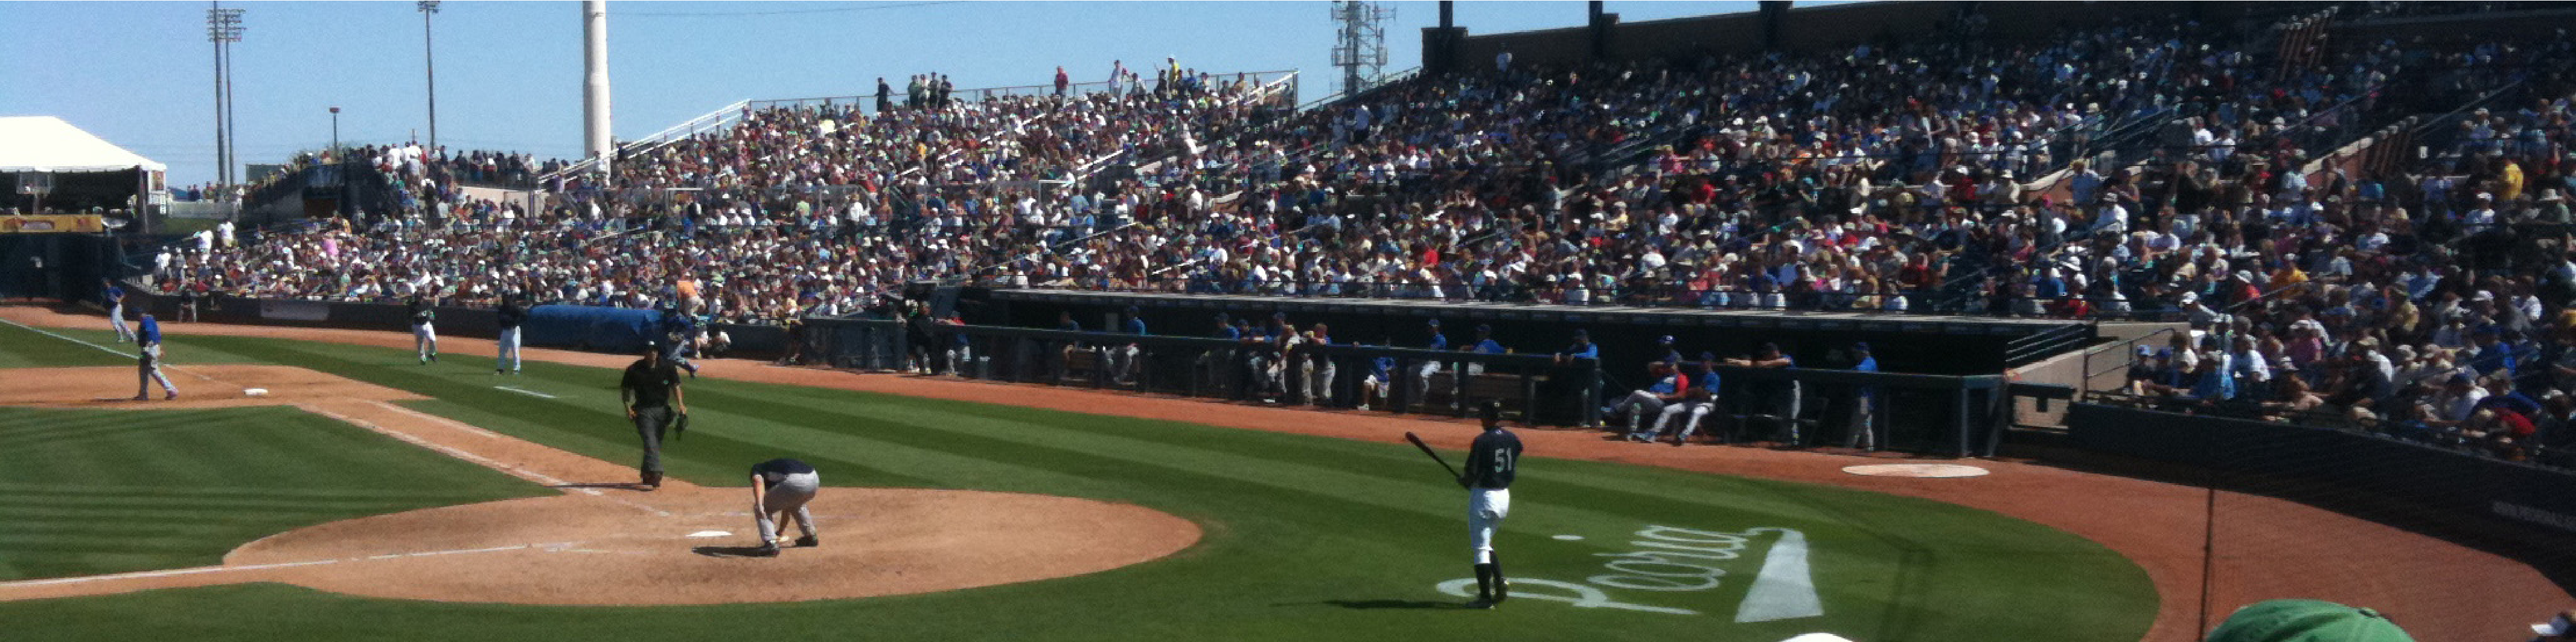
\includegraphics[width=\textwidth]{sampleteaser}
  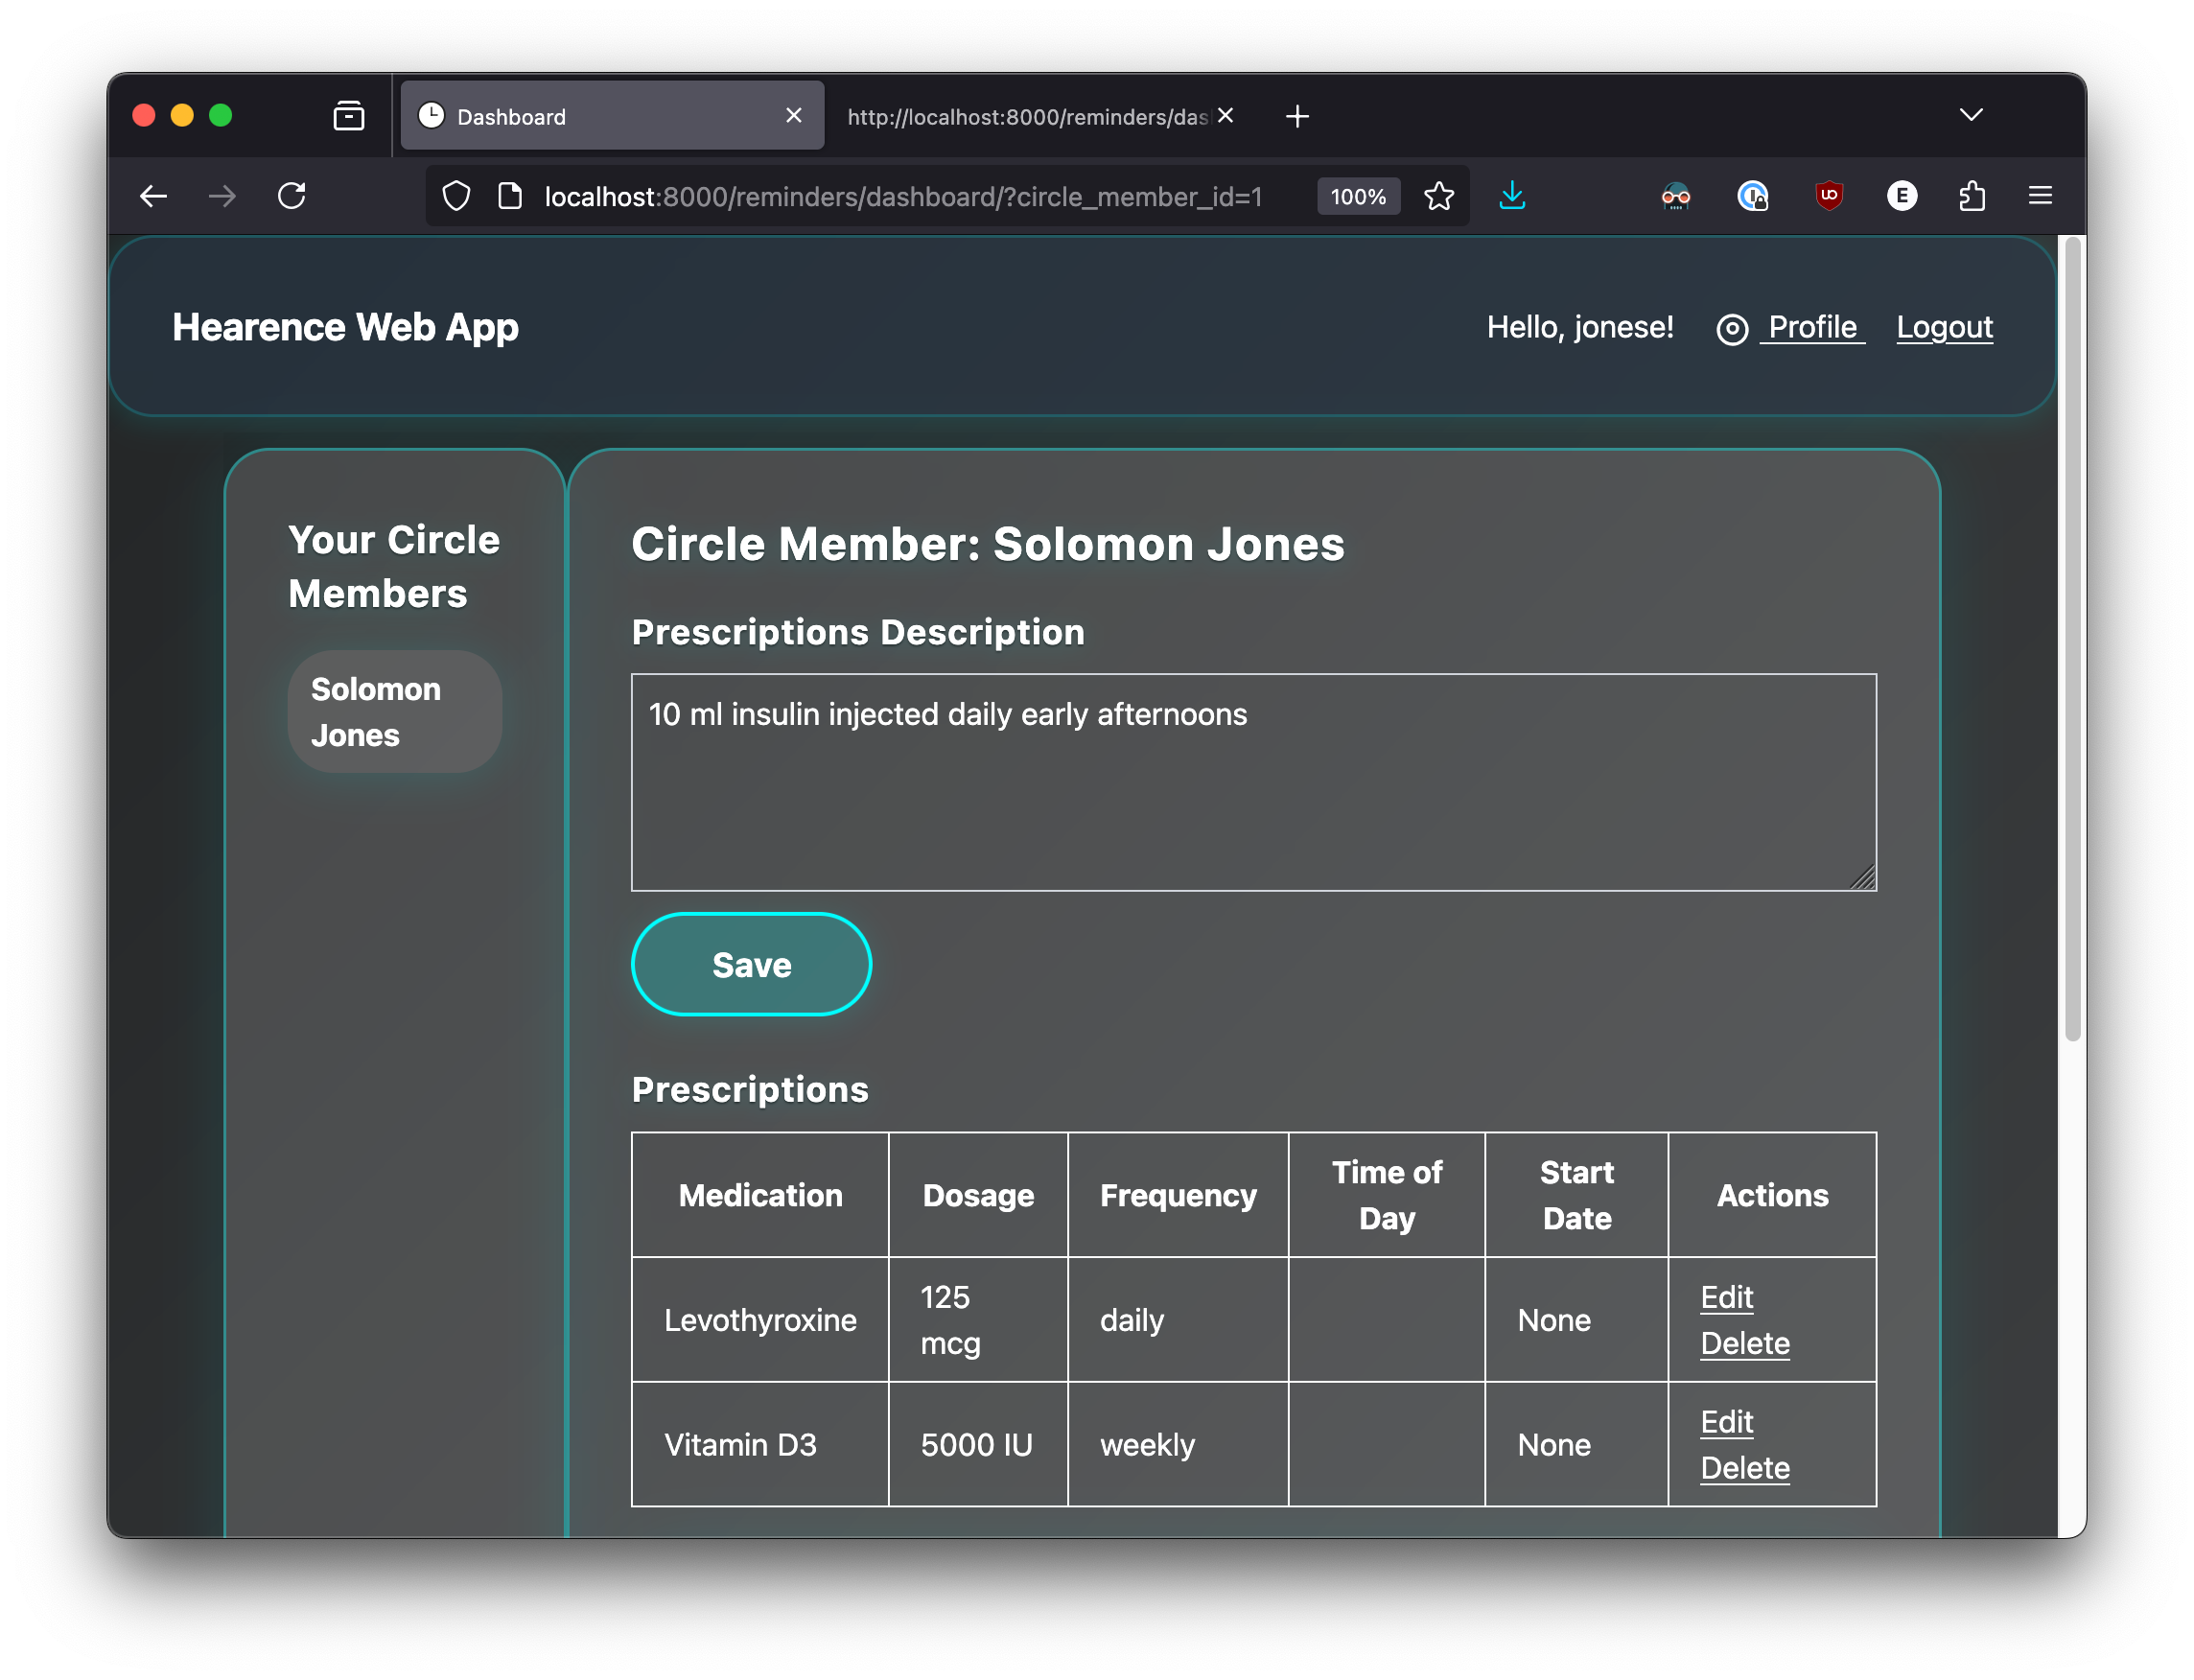
\includegraphics[width=\textwidth]{hearance_web_app_dashboard.png}
  \caption{Hearance web app dashboard.}
  \Description{The basic interface of the Hearance web app.}
  \label{fig:teaser}
\end{teaserfigure}

% FIXME: This was never received, revised, or accepted
% \received{20 February 2007}
% \received[revised]{12 March 2009}
% \received[accepted]{5 June 2009}

%%
%% This command processes the author and affiliation and title
%% information and builds the first part of the formatted document.
\maketitle

\section{Introduction}
This is Evan. Are my citations working? First\cite{Krueger2005}, second, \cite{Wilhelmsen2019}, third, \cite{Gast2019}


Medicine today has developed effective treatments for numerous conditions, yet therapeutic success often hinges not on the efficacy of medications but on whether patients take them as prescribed. Medication adherence—defined as the extent to which patients take medications as prescribed by their healthcare providers—remains a significant challenge in healthcare. This is particularly true for vulnerable populations, including older adults and those with complex medication regimens. Conditions like schizophrenia and diabetes, which are largely manageable with proper medication, continue to cause substantial suffering due to poor adherence.

This project aimed to address the adherence challenge through an innovative approach: leveraging conversational artificial intelligence to create relationship-based medication reminders. Rather than simply alerting patients when to take their medications, our system was designed to engage them in natural conversations, recognizing that people are more likely to respond positively to friendly interactions than to utilitarian reminders.

\section{Background: The Medication Adherence Challenge}
The World Health Organization estimates that approximately 50\% of patients with chronic illnesses do not take medications as prescribed (Sabate, 2003)\cite{Sabate2003}. This problem is even more pronounced in developing countries and among elderly populations. In the United States alone, non-adherence leads to approximately 125,000 deaths annually and accounts for 10\% of hospitalizations (Krueger et al., 2005)\cite{Krueger2005}.

The economic impact is equally staggering, with estimates suggesting that medication non-adherence costs the U.S. healthcare system between $100-$300 billion yearly (Aremu, 2022)\cite{Aremu2022}. These costs stem from increased hospital admissions, disease progression, and additional treatments that might have been avoided with proper medication adherence.

Common barriers to adherence include:

\begin{itemize}
  \item Psychological factors: Denial of illness, fear of side effects, misunderstanding of disease consequences
  \item Practical barriers: Complex regimens, forgetfulness, cost constraints
  \item Educational gaps: Insufficient knowledge about the medication or condition
  \item Relational factors: Poor patient-provider communication and trust
\end{itemize}

As Kardas et al. (2013)\cite{Kardas2013} identified through systematic review, adherence is multifactorial and requires multifaceted interventions to address effectively.

\section{Current Approaches and Their Limitations}

The healthcare industry has implemented various strategies to improve medication adherence:

\begin{itemize}
  \item Standard reminder systems: SMS text messages, alarm clocks, pill organizers
  \item Medication tracking applications: Mobile apps that log medication intake
  \item Smart pill dispensers: Devices that dispense medications at programmed times
\end{itemize}

A comprehensive review by Wilhelmsen and Eriksson (2019)\cite{Wilhelmsen2019} found that technological interventions show promise but often fail to deliver sustained improvements. Many current solutions focus exclusively on the functional aspects of adherence—reminding patients when to take their medications—while neglecting the psychological and relational components.

The gap in current solutions lies in their utilitarian approach. Patients often perceive these tools as impersonal and mechanical, leading to alert fatigue and eventual disengagement. Haynes et al. (2008)\cite{Haynes2008} found that even the most effective interventions produce only modest improvements in adherence rates, suggesting the need for novel approaches that address the human elements of medication-taking behavior.

\section{Project Rationale: The Relationship Hypothesis}

My project was founded on what I call the "relationship hypothesis": the premise that adherence behaviors improve when patients feel they are engaged in a supportive relationship rather than merely following instructions. This hypothesis draws from established psychological principles regarding human motivation and engagement.

Research in healthcare consistently demonstrates that strong provider-patient relationships correlate with improved adherence (Dunbar-Jacob et al., 1991)\cite{DunbarJacob1991}. Patients who feel heard, understood, and supported by their healthcare providers are more likely to follow treatment recommendations. Similarly, social support from family members and caregivers has been shown to significantly improve medication adherence (Col et al., 1990)\cite{Col1990}.

I hypothesized that conversational AI could bridge the gap between impersonal reminders and human relationships by simulating supportive interactions. By creating a system that remembers past conversations, asks about well-being, and responds to concerns rather than simply issuing reminders, I hoped to foster a sense of connection that would motivate adherence behaviors.

\section{Project Design and Implementation}
The project centered around "Hearance," a system designed to create relationship-based medication reminders through conversational AI. The core architecture consisted of:

\begin{itemize}

  \item \textbf{User Management System}: A Django-based web application allowing caregivers to create accounts and manage medication regimens for patients
  \item \textbf{Conversation Engine}: An LLM-powered system designed to engage patients in natural dialogue
  \item \textbf{Scheduling System}: A module for initiating conversations at appropriate times
  \item \textbf{Conversation summation and storage}: After completing conversations, a transcript was made, and then submitted to an LLM for summarization; conversation records and highlights are stored in the Hearance app.
\end{itemize}

For LLM interactions, I used Simon Willison's \texttt{llm} Python package, which offers a flexible interface to various language models. I chose Gemini 2.0 Flash for its extensive 1-million token context window, allowing for rich conversational history without needing to fragment interactions or break up context into multiple API calls.

Conversation design principles included:

\begin{itemize}
  \item Personalization based on patient profile and medication history
  \item Progressive relationship building through memory of past interactions
  \item Empathetic responses to concerns or reported side effects
  \item Natural turn-taking conversation rather than directive communication
  \item Contextual awareness of the patient's condition and medication requirements
\end{itemize}

Significant privacy and security concerns remain, and were unhandled in this project. The current design encourages a (likely more tech-savvy) caregiver to manage a patient's prescriptions and reminders, and to look at summaries of a patient's conversations. While there are precedents for caregiver relationships in medicine, there are a lot of unexplored privacy and liability issues that would have to be handled in a complete system.

\section{Technical Implementation}
The technical implementation involved several interconnected components:

\begin{itemize}
  \item \textbf{Django Application:} "Hearance" provided the core functionality for account creation and prescription management. Developed with assistance from OpenAI's GPT 4.1, the application featured simple interfaces for caregivers to add, edit, or remove prescriptions and set medication schedules.  I attempted to 
    
  \item \textbf{Task Scheduling:} I used Celery for asynchronous task management, which scheduled daily check-in calls according to each patient's medication regimen.
    
  \item \textbf{LLM Integration:} Using the  \texttt{llm} package, I established a connection to Gemini 2.0 Flash, configuring it with prompts designed to create natural, supportive conversations. The system maintained a summary of previous interactions to ensure continuity across conversations.
    
  \item \textbf{Voice Interface:} For the conversation stream, I attempted to use Vocode, an open-source telephony solution. This component was intended to handle bidirectional voice conversations with patients.
\end{itemize}

The most significant difficulty I encountered was with the voice conversation implementation. Despite Vocode's promising features and open-source nature, I faced persistent challenges in establishing reliable bidirectional conversations. The tool's documentation and example code proved insufficient for my needs, and recent development activity has been limited. In retrospect, a commercial service might have provided more reliable functionality despite the additional cost.

\section{Results and Analysis}
The Django application component of the project performed well, providing a stable and functional platform for account management and prescription tracking. The interface successfully allowed for the creation of patient profiles and detailed medication regimens.

However, I hit a significant roadblock in implementing the voice-based conversation system. Despite numerous attempts to configure and troubleshoot the Vocode integration, I was unable to establish reliable voice-based conversations. This limitation prevented me from testing the core hypothesis regarding relationship-based adherence improvement.

Several lessons emerged from this experience:

\begin{enumerate}
\item A phased approach would have been wiser, beginning with text-based conversations before attempting voice interactions
\item While I prioritized voice conversations to accommodate less technologically capable patients, this decision ultimately delayed project implementation
\item Because I got stopped before real conversations could happen, I wasn't able to evaluate and refine the prompts I used to define conversations. I don't really know how well they would have worked
\end{enumerate}

Consequently, I was unable to gather data on:

\begin{itemize}
\item Adherence metrics before and after implementation
\item User engagement statistics
\item Qualitative feedback on the conversation experience
\item Unexpected findings that might have emerged from real-world testing
\end{itemize}

This experience highlights the importance of establishing core functionality before expanding to more complex features, particularly when working with emerging technologies.

\section{Discussion and Future Directions }
Despite the implementation challenges, the project reinforced the theoretical foundation for relationship-based adherence interventions. The technical architecture developed for prescription management remains sound and could serve as a foundation for future work.

For subsequent iterations, I would recommend:

\begin{enumerate}

\item \textbf{Modality Expansion}: Begin with text-based conversations through SMS or instant messaging platforms before advancing to voice interactions
\item \textbf{Commercial Integration}: Consider established commercial voice APIs to ensure reliable conversation quality
\item \textbf{Progressive Testing}: Implement a phased testing approach with small user groups to identify and address issues early
\end{enumerate}
  
The most valuable next step would be a controlled study comparing different adherence approaches:

\begin{itemize}
\item No intervention (control group)
\item SMS-based reminders without interactive elements
\item Hearance-based conversational interchanges
\item Regular conversations with human caregivers (the standard Hearance aims to simulate)
\end{itemize}

Such a study would help validate the relationship hypothesis and quantify the effectiveness of conversational AI compared to both simpler technological interventions and human interactions.

The potential applications of relationship-based health interventions extend beyond medication adherence to areas such as chronic disease management, mental health support, and preventive care. As LLM technology continues to advance, the capacity for natural and supportive health-related conversations will only improve.

\section{Conclusion}
This project explored an innovative approach to medication adherence through conversational AI, focusing on relationship building rather than simple reminders. While technical challenges prevented full implementation of the voice conversation component, the project established a solid foundation for future work in this area.

The conceptual framework, leveraging the human preference for relationship-based interactions to improve health behavior, remains compelling and deserves further exploration. As healthcare continues to grapple with adherence challenges, technology-mediated relationship building represents a potentially promising approach for improving patient outcomes.

The future of medication adherence interventions likely lies not in more sophisticated reminders but in more human-like interactions. By continuing to develop systems that engage patients as people rather than simply as medication recipients, we can work toward a healthcare environment where adherence is improved through connection rather than compliance.

%% The next two lines define the bibliography style to be used, and
%% the bibliography file.
\bibliographystyle{ACM-Reference-Format}
\bibliography{evan_jones_bib}


\end{document}
\endinput
%%
%% End of file `sample-sigconf-authordraft.tex'.
